Humans don’t start their thinking from scratch every second. As you read this essay, you understand each word based on your understanding of previous words. You don’t throw everything away and start thinking from scratch again. Your thoughts have persistence.

Traditional neural networks can’t do this, and it seems like a major shortcoming. For example, imagine you want to classify what kind of event is happening at every point in a movie. It’s unclear how a traditional neural network could use its reasoning about previous events in the film to inform later ones.

Recurrent neural networks address this issue. They are networks with loops in them, allowing information to persist.
\begin{figure}[htbp]
	\centering
	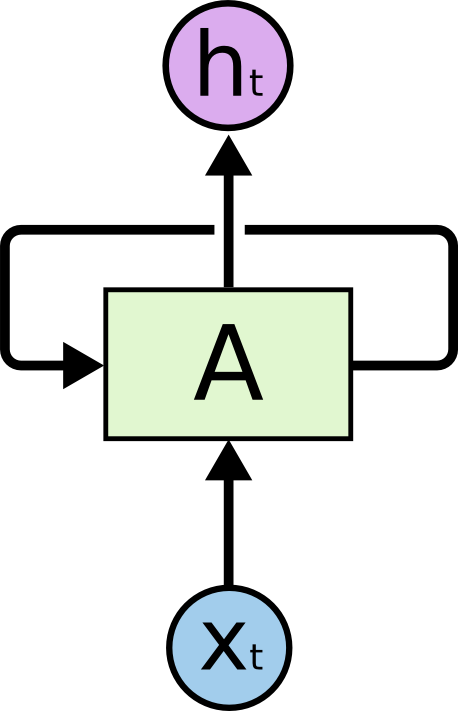
\includegraphics[width=0.15\textwidth]{fig/1.png}
	\caption{Recurrent Neural Networks have loops.}
\end{figure}

In the above diagram, a chunk of neural network, $A$, looks at some input $x_t$ and outputs a value $h_t$. A loop allows information to be passed from one step of the network to the next.

These loops make recurrent neural networks seem kind of mysterious. However, if you think a bit more, it turns out that they aren’t all that different than a normal neural network. A recurrent neural network can be thought of as multiple copies of the same network, each passing a message to a successor. Consider what happens if we unroll the loop:
\begin{figure}[htbp]
	\centering
	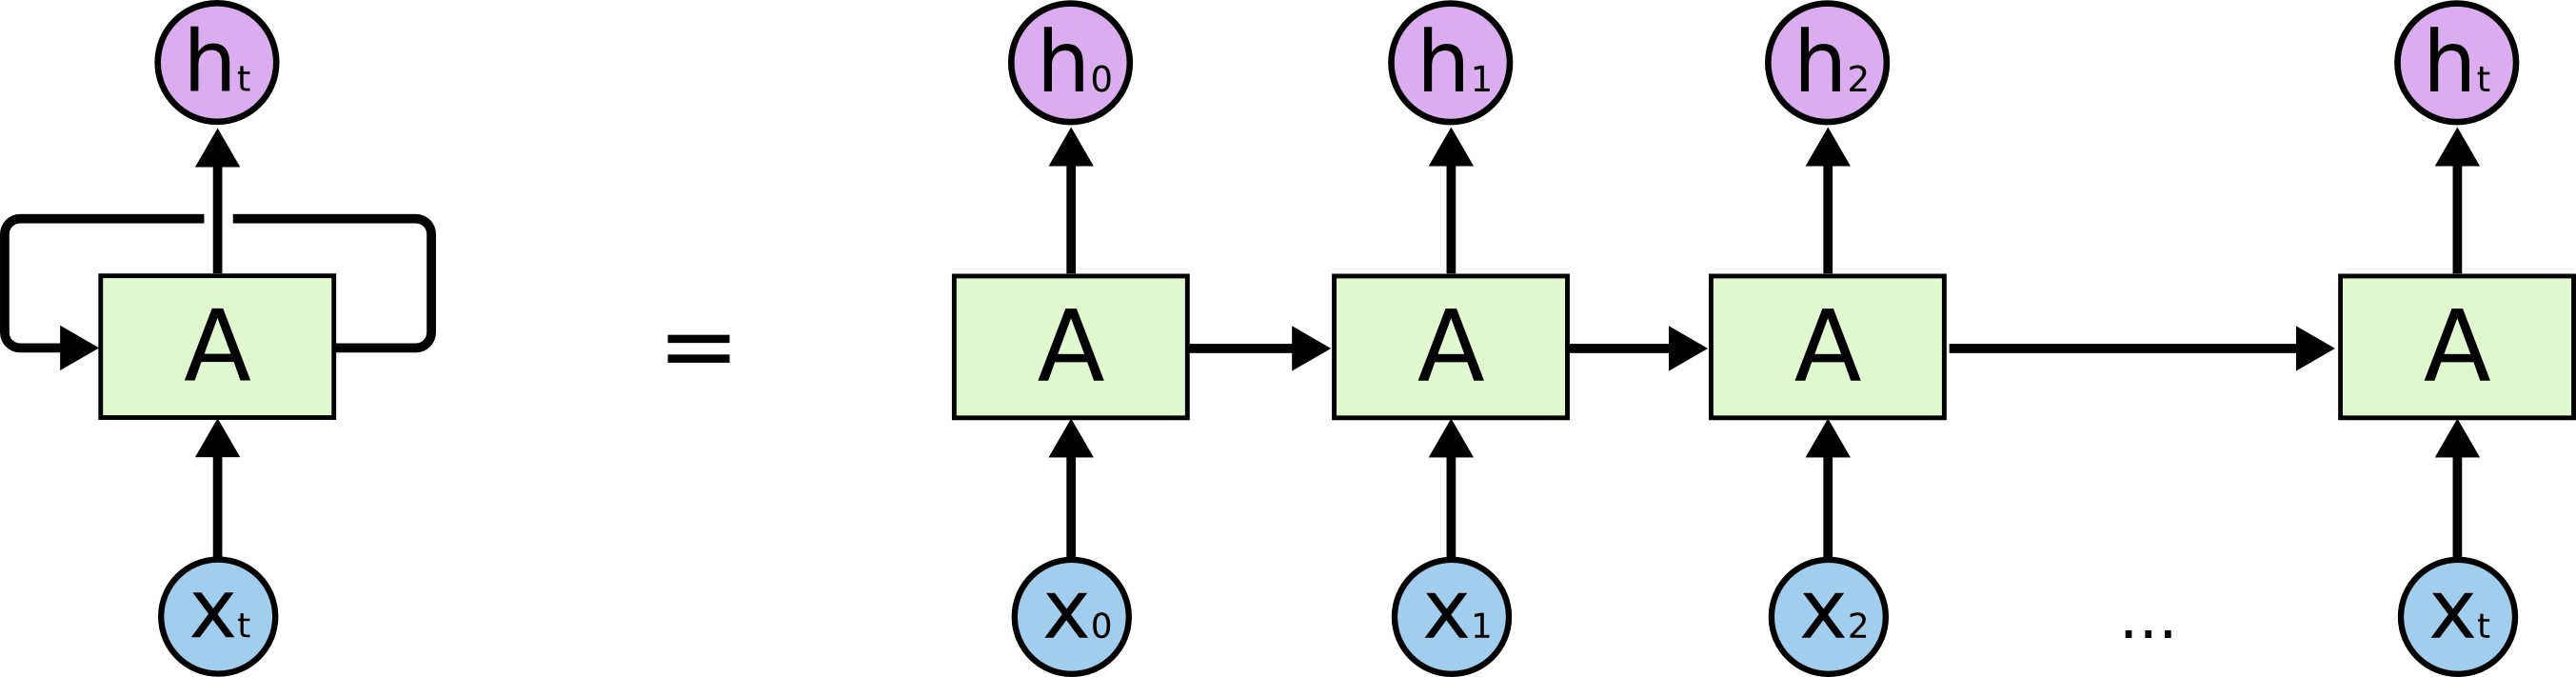
\includegraphics[width=0.75\textwidth]{fig/2.png}
	\caption{An unrolled recurrent neural network.}
\end{figure}

This chain-like nature reveals that recurrent neural networks are intimately related to sequences and lists. They’re the natural architecture of neural network to use for such data.

And they certainly are used! In the last few years, there have been incredible success applying RNNs to a variety of problems: speech recognition, language modeling, translation, image captioning… The list goes on. I’ll leave discussion of the amazing feats one can achieve with RNNs to Andrej Karpathy’s excellent blog post, \href{http://karpathy.github.io/2015/05/21/rnn-effectiveness/}{The Unreasonable Effectiveness of Recurrent Neural Networks}. But they really are pretty amazing.

Essential to these successes is the use of “LSTMs,” a very special kind of recurrent neural network which works, for many tasks, much much better than the standard version. Almost all exciting results based on recurrent neural networks are achieved with them. It’s these LSTMs that this essay will explore.